\chapter{Assembling}



\section{Getting Started With Arduino}
\begin{itemize}
	\item Connect your Arduino Nano board to your laptop and open the control panel. in the control panel, click on Hardware and Sound. Now click on Devices and Printers. Here, find the port to which your microcontroller board is connected.
	\begin{figure}[h]
		\centering
		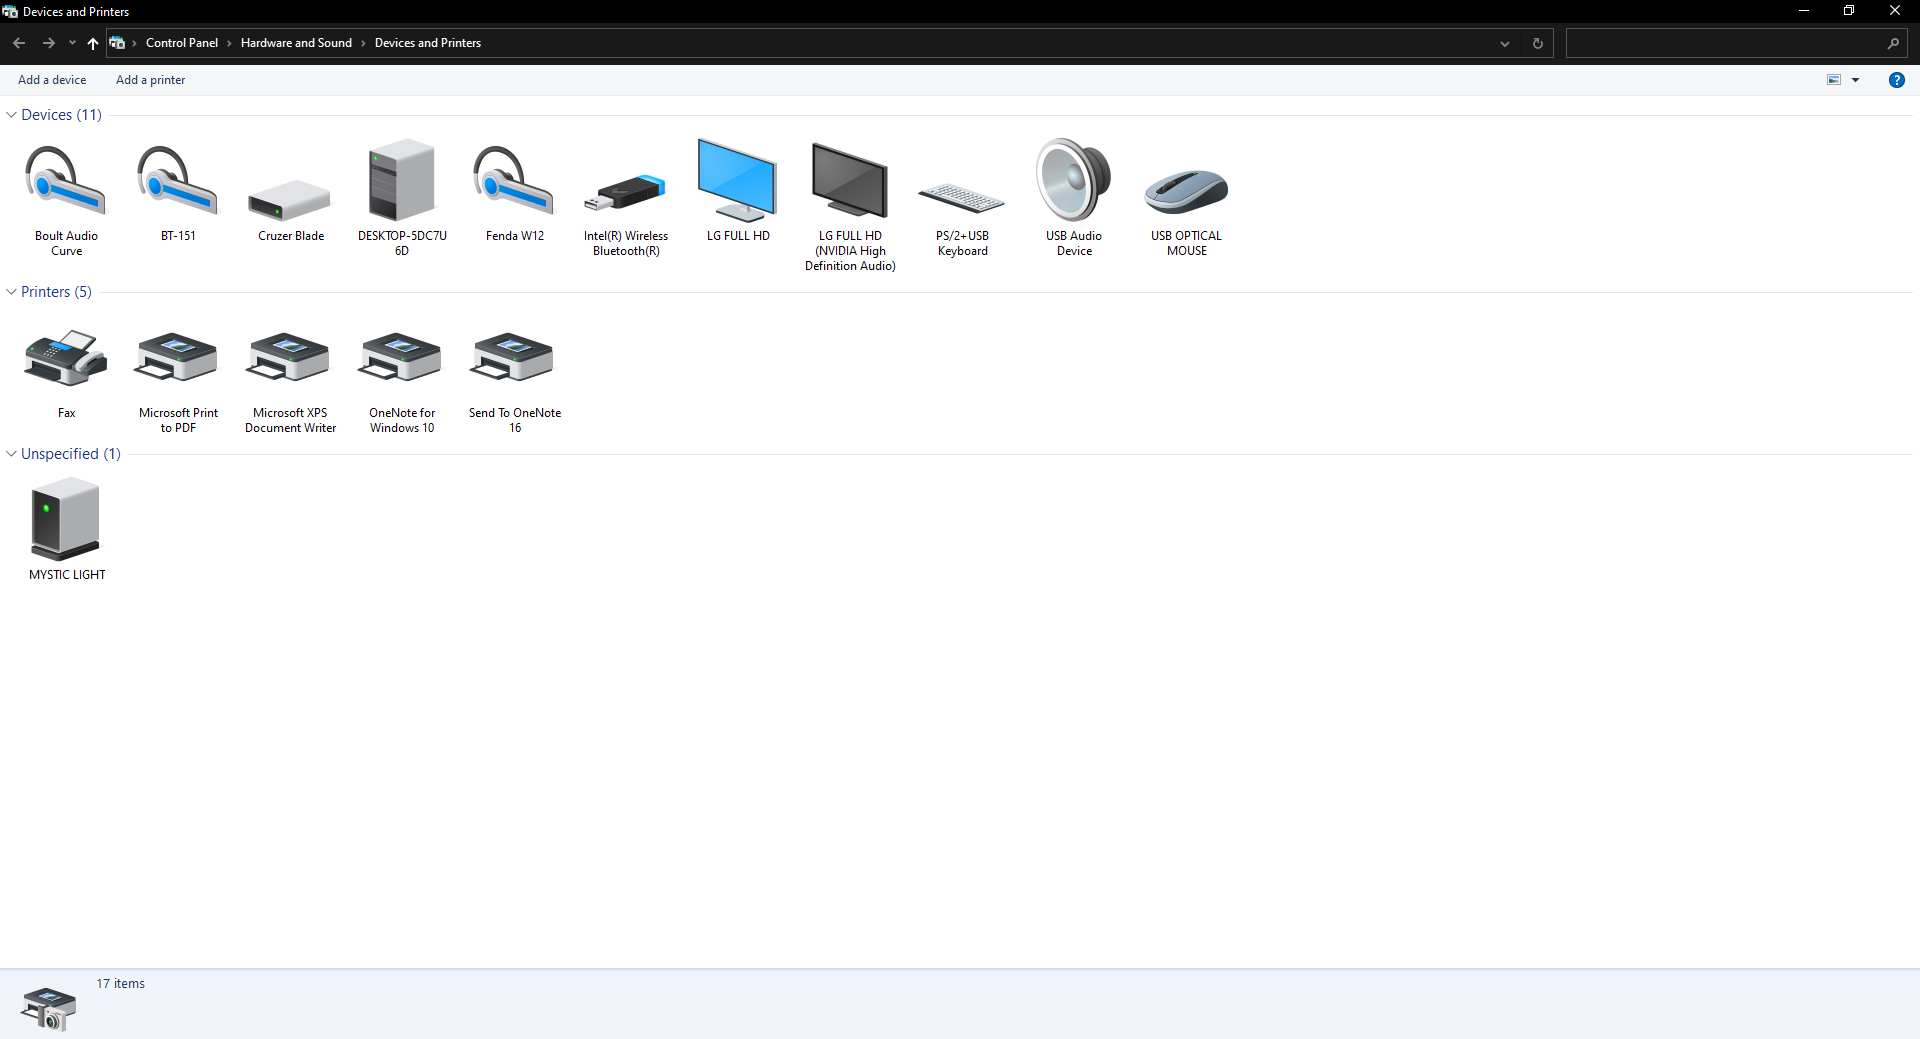
\includegraphics[scale=.35]{Screenshot (17).png}
		\caption{Devices and Printers.}
	\end{figure}
	\item We will have to include a library to use the GSM Module. Go to Sketch > Include Library > Add .ZIP Library.
	\item Click on the Tool menu and set the board to Arduino Nano.
	\begin{figure}[h]
		\centering
		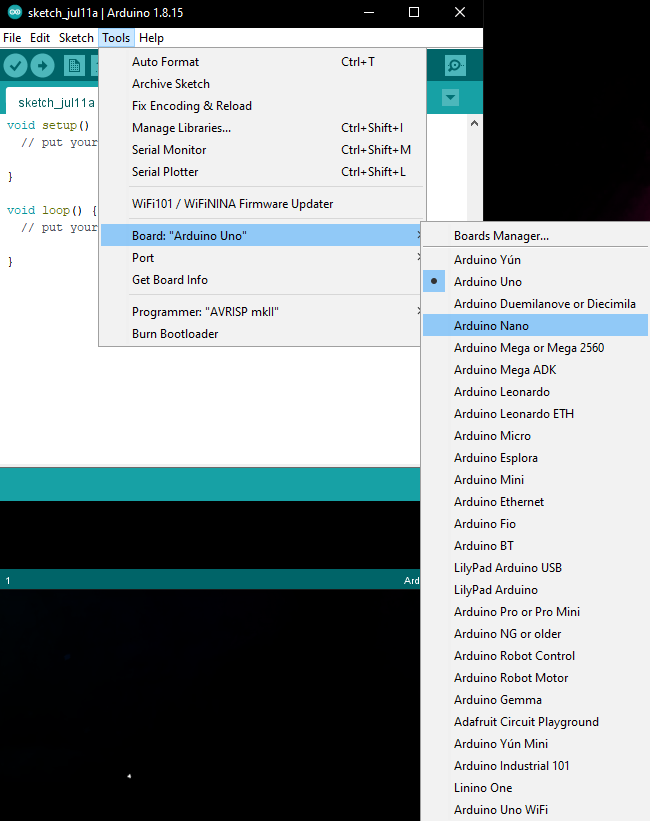
\includegraphics[scale=.48]{Screenshot (19).png}
		\caption{Setting Up Arduino Nano.}
	\end{figure}
	\pagebreak\item In the same Tool menu, Set the Processor to ATmega328P (Old Bootloader).
	\begin{figure}[h]
		\centering
		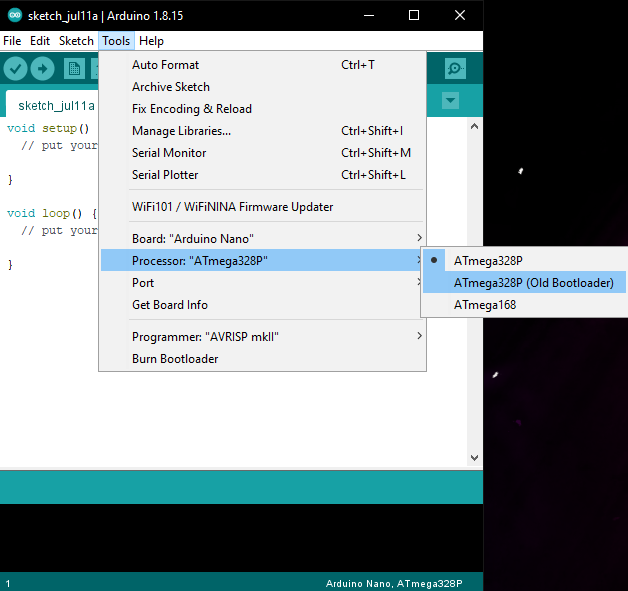
\includegraphics[scale=.45]{Screenshot (21).png}
		\caption{Setting Up ATmega 328P.}
	\end{figure}
	\item Pin 19 of ATmega 328 is connected to pin 13 of Arduino.
	\item Pin 18 of ATmega 328 is connected to pin 12 of Arduino.
	\item Pin 17 of ATmega 328 is connected to pin 11 of Arduino.
	\item Pin 1 of ATmega 328 is connected to pin 10 of Arduino.
	\item Pin 7 of ATmega 328 is connected to Vcc of Arduino.
	\item Pin 8 of ATmega 328 is connected to GND of Arduino.
	\item Pin 9 and 10 of ATmega 328 are connected together with 16 MHz crystal.
	\item In the same Tool menu, set the port to the port number that you observed before in the Devices and Printers.
	\item After that code attached below is pasted into Arduino IDE, the upload button is clicked to burn the code on  microcontroller board.
	
	\begin{figure}[h]
		\centering
		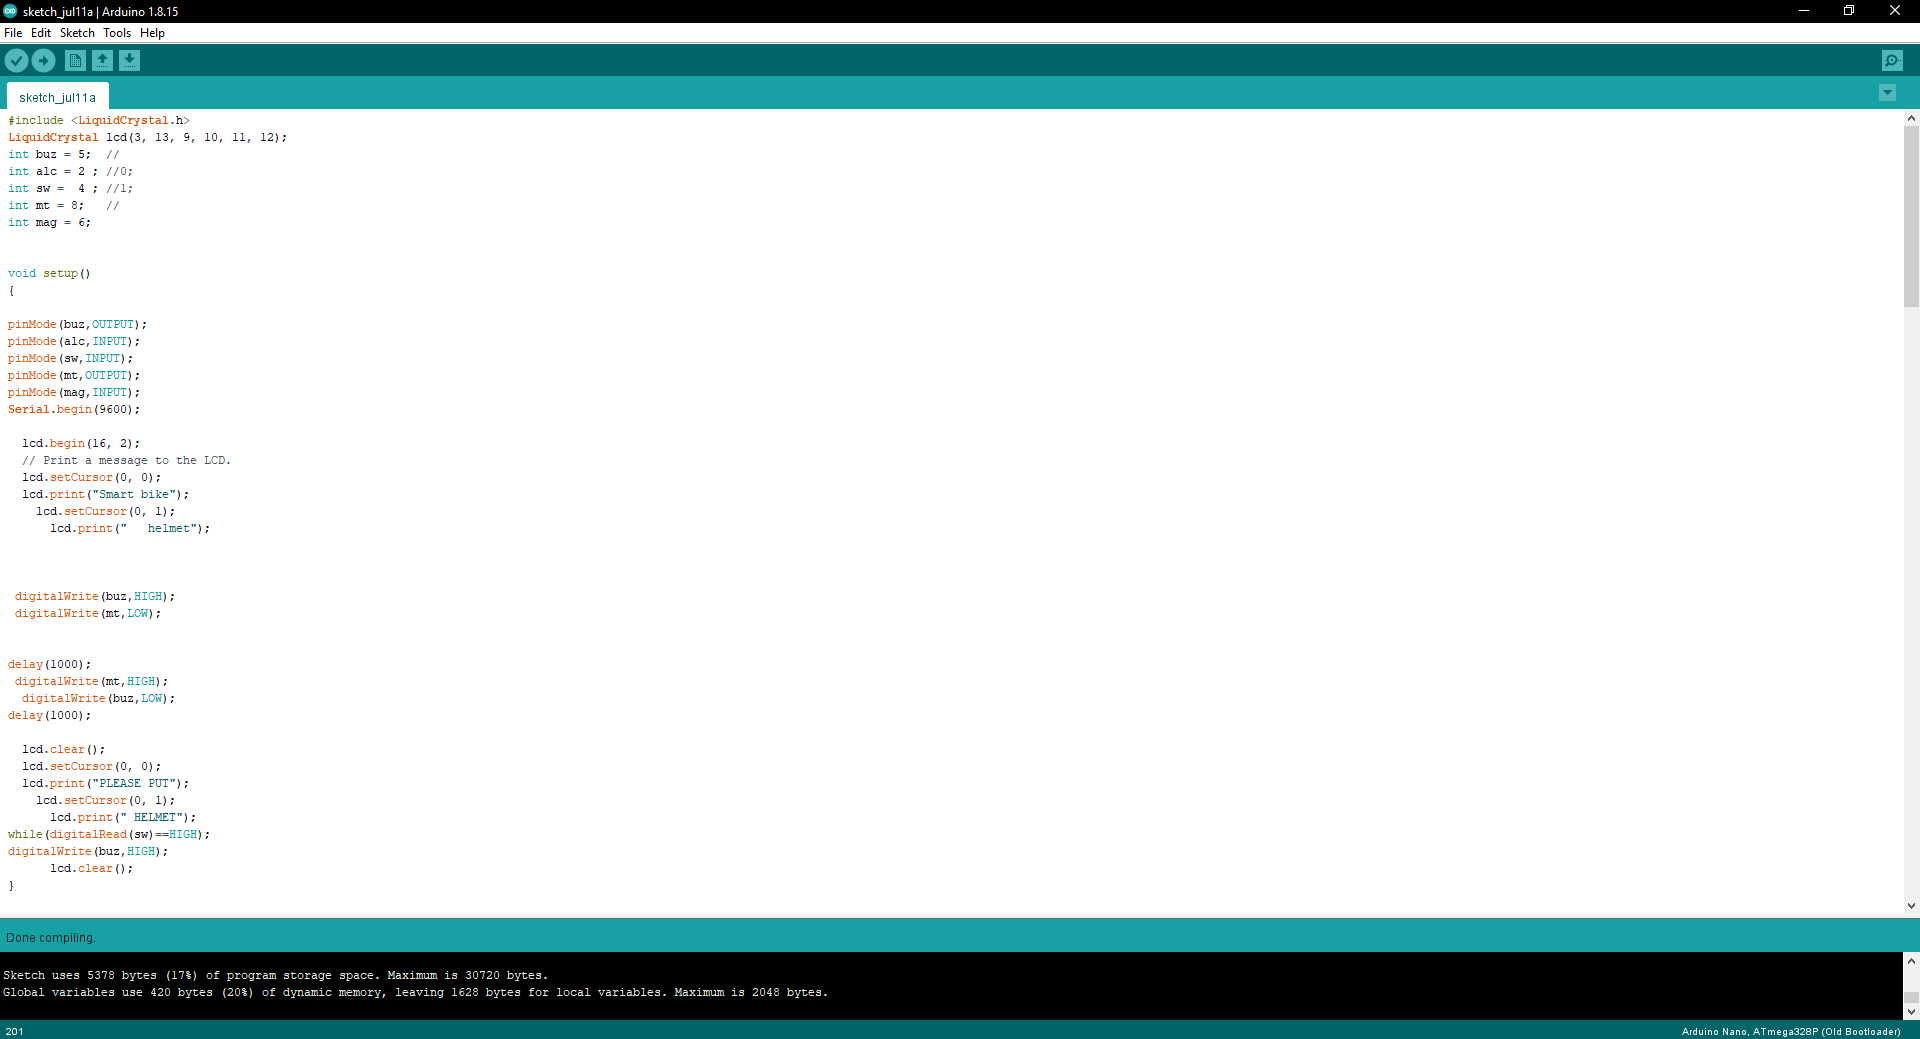
\includegraphics[scale=.35]{Screenshot (23).png}
		\caption{Project Code In Arduino IDE.}
	\end{figure}
	
	
	
	\pagebreak
\end{itemize}


\pagebreak
\section{Code}
\#include $<$LiquidCrystal.h$>$\\
LiquidCrystal lcd(3, 13, 9, 10, 11, 12);\\
int buz = 5;  // \\
int alc = 2 ; //0;\\
int sw =  4 ; //1;\\
int mt = 8;   //\\
int mag = 6;\\
\vspace{.3cm}

void setup()\\
\{ \vspace{.3cm}

pinMode(buz,OUTPUT);\\
pinMode(alc,INPUT);\\
pinMode(sw,INPUT);\\
pinMode(mt,OUTPUT);\\
pinMode(mag,INPUT);\\
Serial.begin(9600);\\
\vspace{.3cm}

lcd.begin(16, 2);\\
// Print a message to the LCD.\\
lcd.setCursor(0, 0);\\
lcd.print("Smart bike");\\
lcd.setCursor(0, 1);\\
lcd.print("   helmet");\\
\vspace{.6cm}


digitalWrite(buz,HIGH);\\
digitalWrite(mt,LOW);\\
\vspace{.3cm}

delay(1000);\\
digitalWrite(mt,HIGH);\\
digitalWrite(buz,LOW);\\
delay(1000);\\
\vspace{.3cm}

lcd.clear();\\
lcd.setCursor(0, 0);\\
lcd.print("PLEASE PUT");\\
lcd.setCursor(0, 1);\\
lcd.print(" HELMET");\\
while(digitalRead(sw)==HIGH);\\
digitalWrite(buz,HIGH);\\
lcd.clear();\\

\} \vspace{.3cm}

//Main Loop To Calculate RPM and Update LCD Display\\
void loop()\\
\{

if(digitalRead(sw)==LOW)\\
\{\vspace{.3cm}

lcd.clear();\\
digitalWrite(mt,LOW);\\
lcd.setCursor(0, 0);\\
lcd.print("IGNITION ON");\\
while( digitalRead(alc)==HIGH \&\& digitalRead(sw)==LOW)\\
\{\vspace{.3cm}

if(digitalRead(mag)==HIGH)\\
\{\vspace{.3cm}

lcd.clear();\\
lcd.setCursor(0, 0);\\
lcd.print("BIKE GOT IN");\\
lcd.setCursor(0, 1);\\
lcd.print("ACCIDENT");\\
init\_sms();\\
send\_data(" YOUR BIKE GOT INTO THE ACCIDENT ");\\
send\_sms();\\
\vspace{.3cm}

delay(5500);\\
\}\vspace{.3cm}

else\\
\{\vspace{.3cm}

\}  \vspace{.3cm}

\}\vspace{.3cm}

\}\vspace{.3cm}

if(digitalRead(sw)==HIGH)\\
\{     lcd.clear();\\
lcd.setCursor(0, 0);\\
lcd.print("               ");\\
lcd.setCursor(0, 0);\\
lcd.print(" NO HELMET ");\\
\vspace{.3cm}


digitalWrite(buz,HIGH);\\
delay(500);\\
digitalWrite(buz,LOW);\\
delay(500);\\
digitalWrite(buz,HIGH);\\
delay(500);\\
digitalWrite(buz,LOW);\\
delay(500);\\
digitalWrite(buz,HIGH);\\
delay(500);\\
digitalWrite(buz,LOW);\\
delay(500);\\
digitalWrite(buz,HIGH);\\
delay(500);\\
\vspace{.3cm}

if(digitalRead(sw)==HIGH)\\
\{  \vspace{.3cm}

digitalWrite(mt,HIGH);\\
while( digitalRead(alc)==HIGH \&\& digitalRead(sw)==HIGH)\\
\{\vspace{.3cm}

if(digitalRead(mag)==HIGH)\\
\{\vspace{.3cm}

lcd.clear();\\
lcd.setCursor(0, 0);\\
lcd.print("BIKE GOT IN");\\
lcd.setCursor(0, 1);\\
lcd.print("ACCIDENT");\\

init\_sms();\\
send\_data(" YOUR BIKE GOT INTO THE ACCIDENT ");\\
send\_sms();\\

delay(5500);\\
\} \vspace{.3cm}

else\\
\{\vspace{.3cm}

\}\vspace{.3cm}

\}\vspace{.3cm}

\}\vspace{.3cm}

\}\vspace{.3cm}

if(digitalRead(alc)==LOW)\\
\{  lcd.clear();\\
lcd.setCursor(0, 0);\\
lcd.print("               ");\\
lcd.setCursor(0, 0);\\
lcd.print("ALCOHOL DETECTED");\\

digitalWrite(buz,HIGH);\\
delay(500);\\
digitalWrite(buz,LOW);\\
delay(500);\\
digitalWrite(buz,HIGH);\\
delay(500);\\
digitalWrite(buz,LOW);\\
delay(500);\\
digitalWrite(buz,HIGH);\\
delay(500);\\
digitalWrite(buz,LOW);\\
delay(500);\\
digitalWrite(buz,HIGH);\\
delay(500);\\

if(digitalRead(alc)==LOW)\\
\{  \vspace{.3cm}

digitalWrite(mt,HIGH);\\
while( digitalRead(alc)==LOW )\\
\{\vspace{.3cm}

if(digitalRead(mag)==HIGH)\\
\{
lcd.clear();\\
lcd.setCursor(0, 0);\\
lcd.print("BIKE GOT IN");\\
lcd.setCursor(0, 1);\\
lcd.print("ACCIDENT");\\
init\_sms();\\
send\_data(" YOUR BIKE GOT INTO THE ACCIDENT ");\\
send\_sms();\\

delay(5500);\\
\} \vspace{.3cm}

else\\
\{\vspace{.3cm}


\} \vspace{.3cm}

\}\vspace{.3cm}

\}\vspace{.3cm}

\}\vspace{.3cm}

\}\vspace{.3cm}


void init\_sms()\\
{\vspace{.3cm}
	
	Serial.println("AT+CMGF=1");\\
	delay(200);\\
	Serial.println("AT+CMGS=$\backslash$"+91XXXXXXXXXX$\backslash$"");   \\
	delay(200);\\
}\vspace{.3cm}

void send\_data(String message)\\
{\vspace{.3cm}
	Serial.println(message);\\
	delay(200);\\
}\vspace{.3cm}

void send\_sms()\\
{\vspace{.3cm}
	
	Serial.write(26);\\
}\vspace{.3cm}
